
\section{\textbf{Emperical Results}}
    We compare QPAIR and QSCAN with state-of-the-art MARL approaches, QMIX and QPLEX, in various coordination tasks, including matrix games, predator-prey challenges \cite{r8}, the Switch task \cite{r6}, and the StarCraft Multi-Agent Challenge (SMAC) \cite{r7}. For a fair comparison, the implementation of QSCAN uses one attention layer, that is, with sub-teams of size 2. The learning curves are plotted with a smooth factor of 0.6 except the last point. The implementation detail and environment detail are in Appendix C. 


    \subsection{Matrix Game}
    \begin{wraptable}{r}{.7\textwidth}
        \caption{Payoffs of a 3-player matrix game. Each player \emph{i} $\in$ \{ 1,2,3 \} has two actions \{ A,B \}.The complete payoff matrix is split into two submatrices according to player 1’s action a1.}
        \vspace{10pt}
        \begin{tabular}{cc}
             \begin{tabular}{c}
                 when $a_1=A$ \\[2ex]
                \begin{tabular}{|l||*{2}{c|}}\hline
                    \backslashbox{$a_{2}$}{$a_{3}$}
                    &\makebox[3em]{A}&\makebox[3em]{B}\\\hline\hline
                     A &0 &0\\\hline
                     B &\textbf{23}&12\\\hline
                \end{tabular}
             \end{tabular}
             &
             \begin{tabular}{c}
                 when $a_1=A$ \\[2ex]
                \begin{tabular}{|l||*{2}{c|}}\hline
                    \backslashbox{$a_{2}$}{$a_{3}$}
                    &\makebox[3em]{A}&\makebox[3em]{B}\\\hline\hline
                     A &17 &20\\\hline
                     B &03&17\\\hline
                \end{tabular}
             \end{tabular}
        \end{tabular}
        \label{tab:pay}
    \end{wraptable}

    Table ~\ref{tab:pay} shows the payoffs of a 3-player with 2-action matrix game. Fig ~\ref{fig:sub_learning_a} illustrates the empirical results for QMIX, QPLEX, QPAIR and QSCAN. Due to the relative overgeneralization,fails to find the optimal solution. QPLEX suffers another problem about the poor generalization. QSCAN and QPAIR can find the optimal solution more quickly because the pairwise coordination patterns provide more suitable generalization in this task. In the exploration period ,The pairwise coordination would allow the algorithm to explore the optimal solution more easily. Moreover, for all different random seeds in our experiments, QSCAN always finds the optimal solution rapidly in this matrix game.



    \begin{figure}[htbp]
        \centering
        \begin{subfigure}[b]{0.3\textwidth}
            \centering
            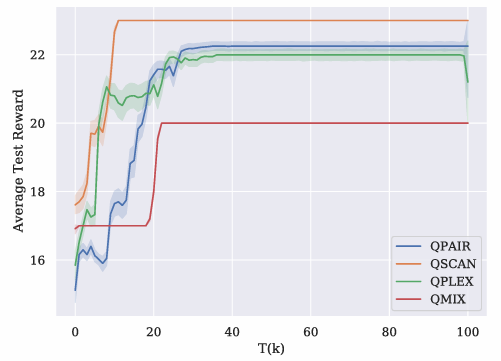
\includegraphics[width=\textwidth]{images/ima1.png}
            \caption{Matrix game.}
            \label{fig:sub_learning_a}
        \end{subfigure}
        \hfill
        \begin{subfigure}[b]{0.3\textwidth}
            \centering
            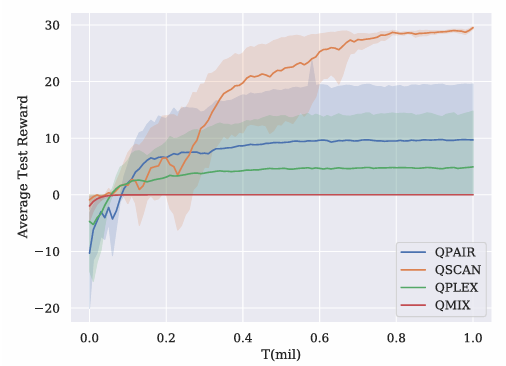
\includegraphics[width=\textwidth]{images/ima2.png}
            \caption{Predator-Prey (6 versus 6).}
            \label{fig:sub_learning_b}
        \end{subfigure}
        \hfill
        \begin{subfigure}[b]{0.3\textwidth}
            \centering
            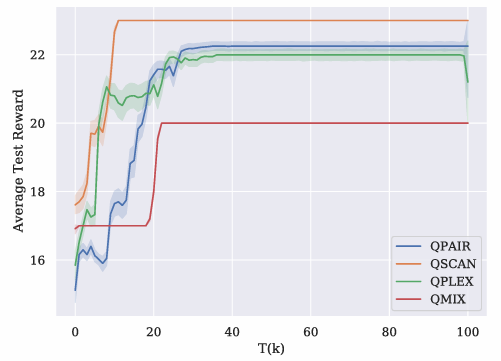
\includegraphics[width=\textwidth]{images/ima1.png}
            \caption{Switch4 challenge.}
            \label{fig:sub_learning_c}
        \end{subfigure}
        \caption{Learning curves of QPAIR, QSCAN, QPLEX, and QMIX in three different tasks. For the timestamp T, k and mil are short for 1s 'kilo' and 'million' respectively. The shaded area with 95\% confidence intervals is shown. Best viewed in color.}
        \label{fig:learning_curves}
    \end{figure}


    % \pagebreak

    \subsection{\large{TheStarCraft Multi-Agent Challenge}}

    \begin{wraptable}{r}{.6\textwidth}
        \caption{ Median of the test win rates in the SMAC.}
        \label{tab:tab2}
        \begin{tabular}{cccccc}
            \hline
            Scenario & QSCAN & QPAIR & QPLEX & QMIX \\
            \hline
            2s\_vs\_1sc & \textbf{100} & \textbf{100} & \textbf{100} & \textbf{100} \\
            2s3z & \textbf{100} & \textbf{100} & \textbf{100} & 97 \\
            3s5z & \textbf{98} & 97 & 97 & 94 \\
            1c3s5z & 88 & \textbf{97} & \textbf{97} & 94 \\
            2c\_vs\_64zg & 62 & 86 & \textbf{88} & 42 \\
            5m\_vs\_6m & \textbf{76} & 77 & 72 & 69 \\
            \hline
        \end{tabular}
    \end{wraptable}

    The StarCraft Multi-Agent Challenge (SMAC)\cite{r7} is a widely-used benchmark for cooperativeMARL.Weevaluate our approaches on a widerange of SMAC scenarios, including homogeneous (e.g., 5mvs6m) and heterogeneous (e.g.,3s5z) agents. Furthermore, we compare our approaches with state-of-the-art baselines: QMIX and QPLEX. The empirical results are shown in Table ~\ref{tab:tab2}, and the corresponding figures are presented in Appendix E.4.\\
    
        The results shows that \textbf{QSCAN} and \textbf{QPAIR} are superior to \textbf{QMIX} in most scenarios. QSCAN performs 
        almost well except for 2c\_vs\_64zg. Its win rate is about 20\% less than that of QPAIR or QPLEX. 
        2c\_vs\_64zg needs the coordination of two colossi, where the pairwise coordination characterized 
        by QPAIR coincides with the grand team coordination characterized by QPLEX. As QMIX does not 
        perform well in this scenario, we conjecture that this scenario requires the pairwise coordination 
        patterns rather than individual patterns. One possible reason for the performance of QSCAN could be 
        that the individual patterns through the residue links prevent QSCAN to achieve better performance in 
        this scenario. QPAIR achieves the best performance in some scenarios and no more than 2\% less 
        than the best one's win rate in other selected scenarios. Overall, our approaches achieve comparable 
        performances with the SOTA baseline QPLEX which uses the joint action in the mixing net.